\label{sec:meminj}
\subsection{Memory injection in CompCert}

To prove the correctness of many passes, CompCert uses memory injections. Informally, memory injections are relations between two memories that are true when the two memories are similar. For instance, this is used when doing optimizations, to show that the memory of the source program is similar to the memory of the optimized programs.

In CompCert, memory injection are parametrized with an \textit{injection function}, of type \texttt{block -> option(block * Z)}. This function establish a correspondence between blocks of the source memory and blocks of the target memory.
Informally, if $f(b_1)=\text{Some}(b_2,o)$, then the block $b_1$ in the source memory corresponds to the block $b_2$ in the target memory, with a shift in offsets of $o$. The values are preserved between the two blocks, and the pointers are modified to reflect the eventual change of logical address.
The injection function also define \textit{private} and \textit{public memory}. Public memory is the set of blocks that are mapped to some other block. These blocks should be preserved by optimizations.
Private memory is the set of blocks that are mapped to \texttt{None}. These blocks are only privately used and can be changed separately.
For instance, when performing an unknown external call in both the source and target programs, CompCert assumes that it preserves the memory injection. Thus, the new public memories are equivalent but the call may have changed the private part.

\subsection{Memory injection in the quasi-concrete model}

\begin{figure}
\begin{minipage}{0.5\textwidth}
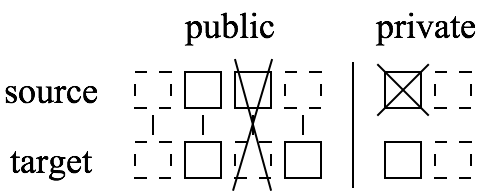
\includegraphics[scale=0.35]{img/meminj.png}
\end{minipage}\quad\quad
\begin{minipage}{0.5\textwidth}
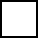
\includegraphics[scale=0.35]{img/concrete.png} Concrete block\\
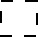
\includegraphics[scale=0.35]{img/logical.png} Logical block
\end{minipage}
\caption{Memory Injection, taken from~\cite{DBLP:conf/pldi/KangHMGZV15}}
\label{fig:meminj}
\end{figure}

As described in~\cite{DBLP:conf/pldi/KangHMGZV15}, memory injection using the quasi-concrete model should be stronger.

To preserve behavior refinement, any successful memory access in the source memory should succeed as well in the target memory. This has several consequences (Fig.~\ref{fig:meminj}).
Firstly, when a source concrete block is mapped to another target block with a given offset in a memory injection, the target should be concrete and their concrete addresses should differ with the same offset.
Finally, there should be no concrete block in the source's private memory.
Formally:
$$\forall b_1,b_2,o,p,\quad f(b_1)=(b_2,o)\wedge b_1\text{ has address }p\implies b_2\text{ has address }p+o$$
$$\forall b_1,\quad f(b_1)=\texttt{None}\implies b_1\text{ has address }\texttt{None}$$

These two properties have been added to CompCert's memory injection. The proofs of every memory injection in CompCert have been updated.

The new implementation can be found in Appendix, section~\ref{subsec:injectimplem}.
